%************************************************
\chapter{Design}\label{ch:design}
%************************************************
%\glsresetall % Resets all acronyms to not used

The software design for each sprint is done ahead of the respective sprint.
This procedure goes along well with the Agile Manifesto which
encourages the design of a complex system in small incremental parts.

\subsection{Sprint 1: PSK31 and RDS demodulation}

The existing architecture of \ac{AnSiAn} features individual threads for scheduling, 
downsampling, demodulation and audio output. The \texttt{De\-mo\-du\-la\-tor} thread demodulates 
quadrature samples by calling the \texttt{demodulate()} method on an instance of
\texttt{Demodulation}. \texttt{Demodulation} is an abstract class that is implemented by concrete 
demodulation methods such as \texttt{AM}, \texttt{FM} and \texttt{Morse}. 

\ac{AnSiAn} utilizes the EventBus library in order to pass demodulated Morse text
to the \ac{GUI}. Demodulated audio data is passed to the
\texttt{AudioSink} thread by enqueuing it into its input queue.
This mechanism is explained in more detail in \autoref{sec:cleanup.mem}.


In order to extend \ac{AnSiAn} with demodulation functionality for \ac{PSK31} and \ac{RDS}, 
the existing architecture needs to be extended. The extended architecture is
depicted in \autoref{fig:demod_text_eventbus} and explained in the following.

\begin{figure}
	\centering
	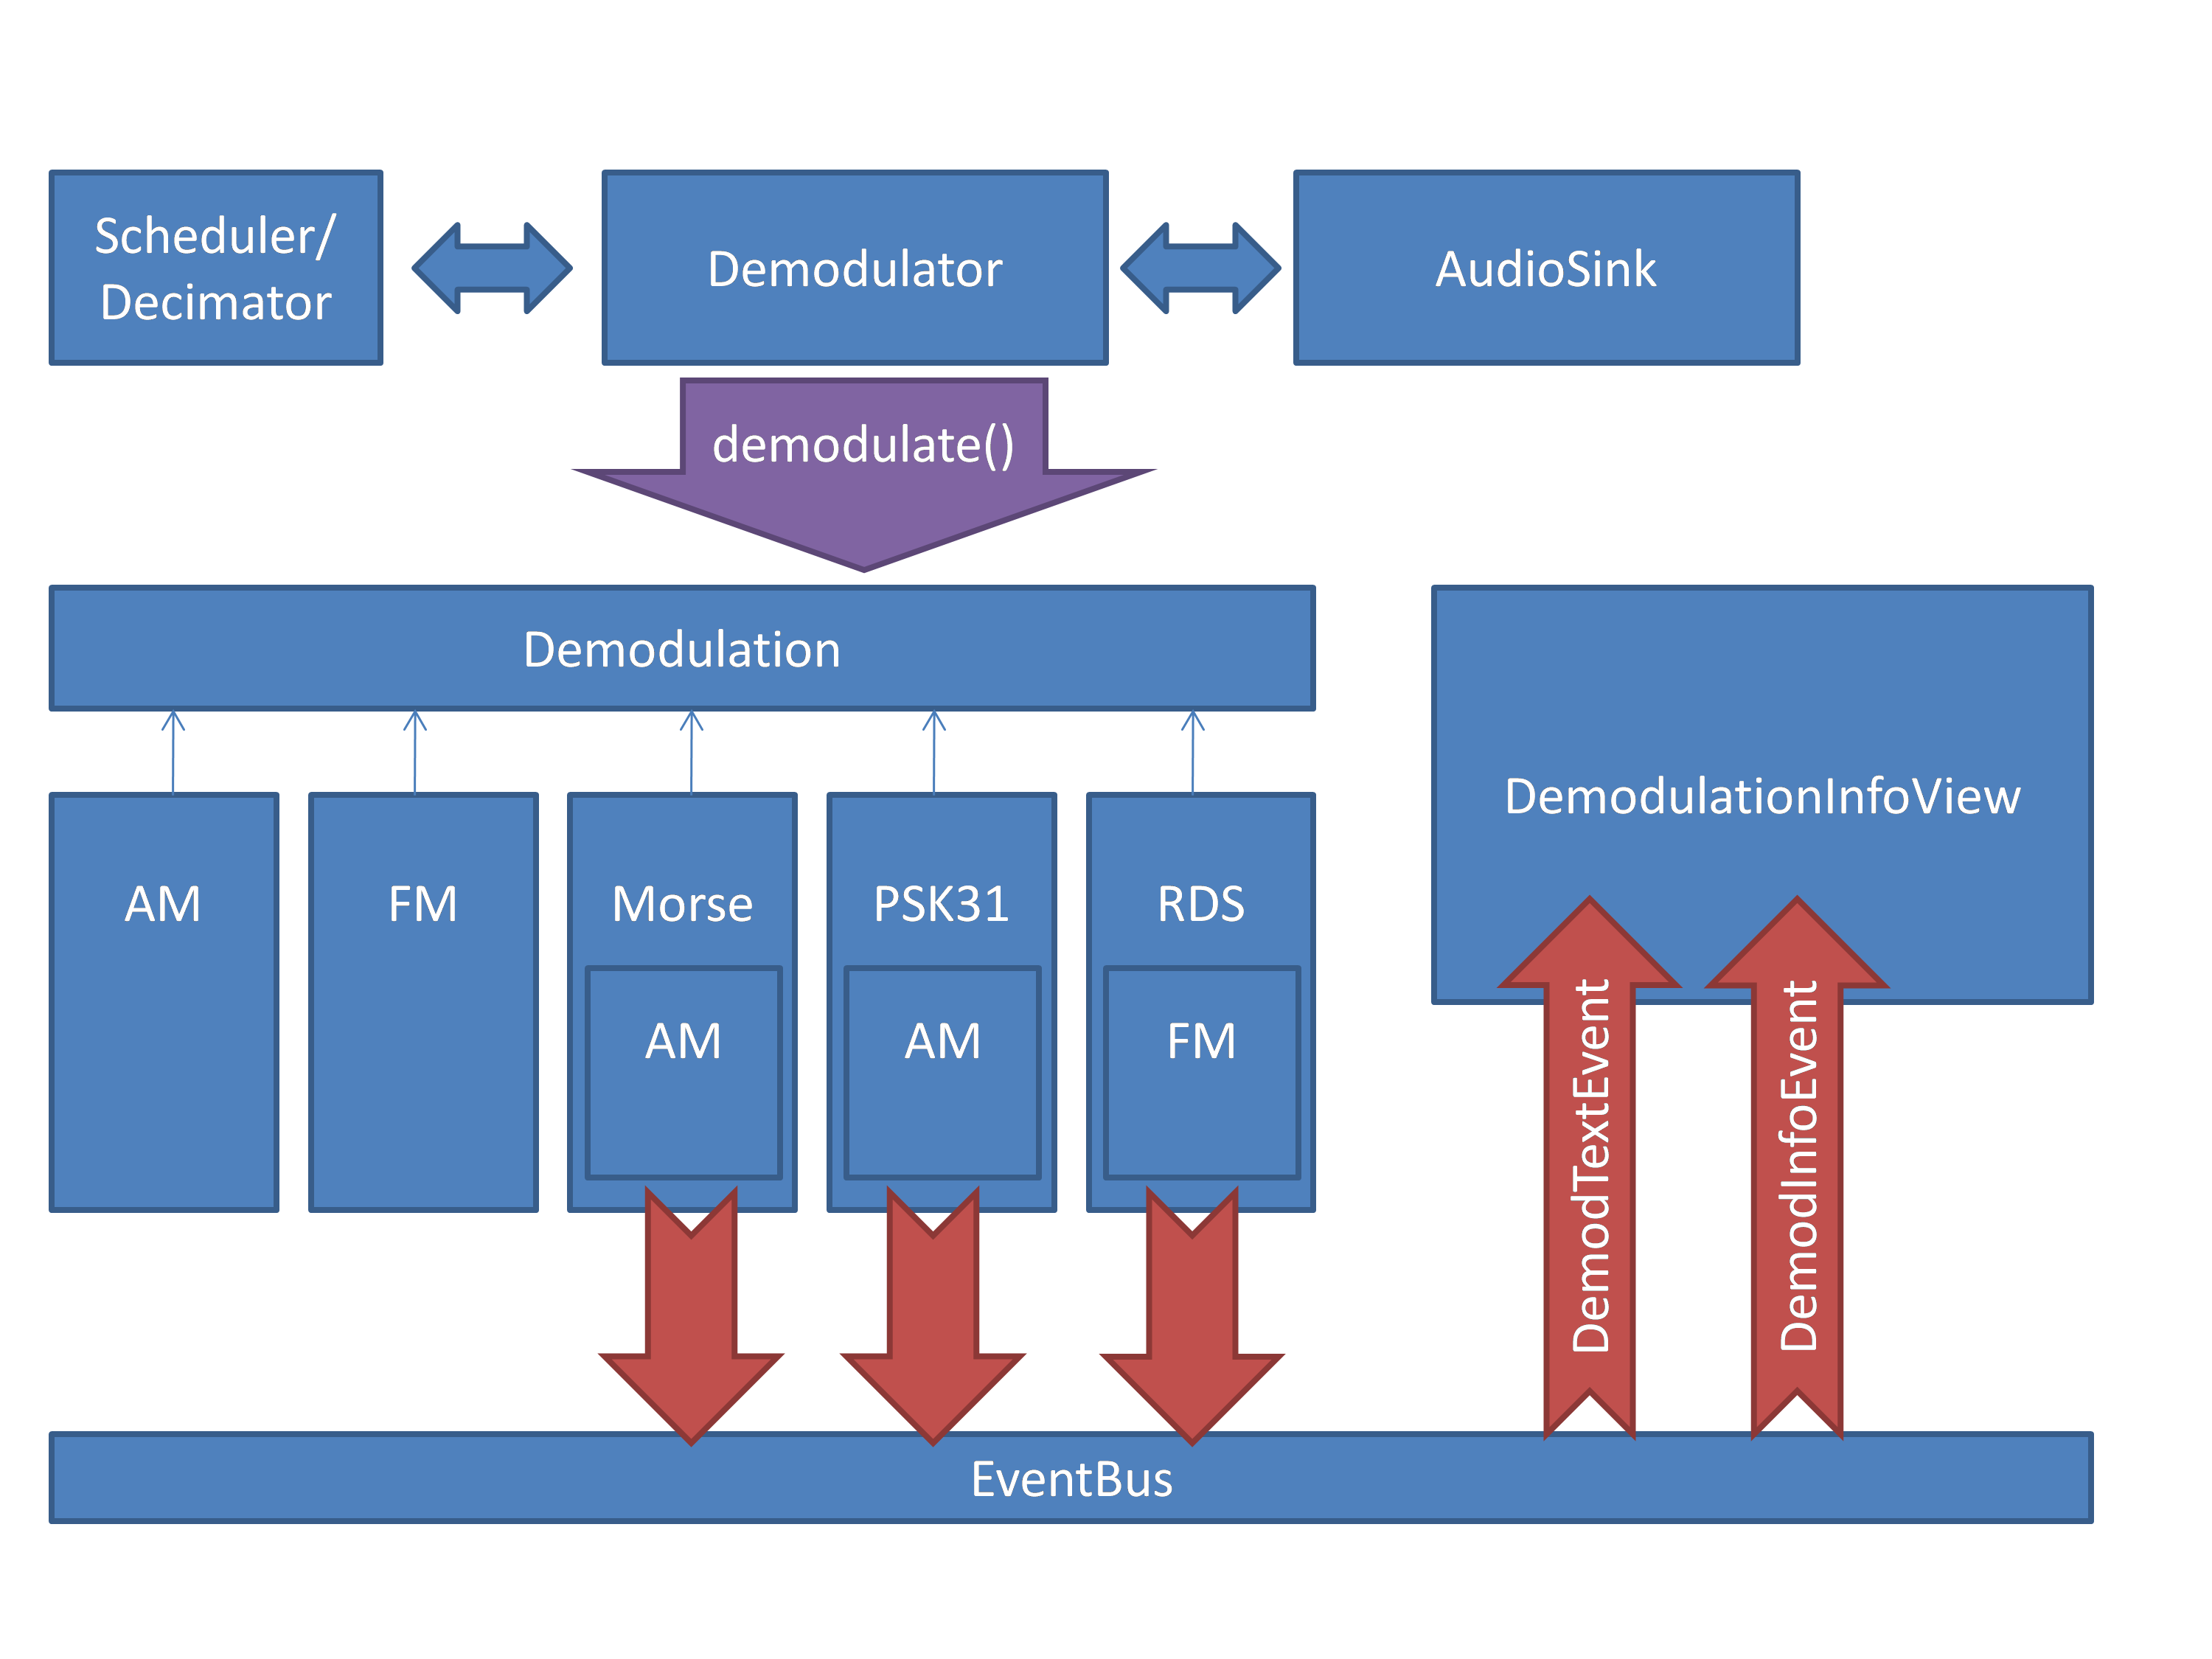
\includegraphics[width=1\linewidth]{gfx/demod_text_eventbus.png}
	\caption{Architecture of the extended demodulation logic and communication with the GUI}
	\label{fig:demod_text_eventbus}
\end{figure}

Two new classes \texttt{PSK31} and \texttt{RDS}, that inherit from
\texttt{Demodulation}, need to be implemented to represent the new demodulation 
mechanisms.

As \ac{PSK31} demodulation works on the envelope of the received signal
and \ac{AM} demodulation essentially performs envelope detection, \texttt{PSK31}
uses an instance of \texttt{AM} for envelope detection.

\ac{RDS} transmits metadata for \ac{FM} radio channels. It is therefore desirable for the 
\ac{RDS} demodulation mode to not only display this metadata, but to also play the 
\ac{FM}-modulated audio at the same time. The \texttt{RDS} class uses an
instance of \texttt{FM} for this purpose.

Like the existing architecture, the new architecture will use the EventBus
library to pass the demodulated text to the \ac{GUI}. The existing View
\texttt{MorseReceiveView} is refactored into a universal
\texttt{De\-mo\-du\-la\-tion\-In\-fo\-View} that displays the text output of any selected 
demodulator. Demodulators pass \texttt{DemodTextEvent}s and 
\texttt{DemodInfoEvent}s via the EventBus to the \texttt{De\-mo\-du\-la\-tion\-In\-fo\-View}, 
which contain demodulated text and further information (e.g. baud rates or raw 
dits and dahs) and are displayed in separate lines.

%************************************************
\chapter{Implementation}\label{ch:implementation} % $\mathbb{ZNR}$
%************************************************
%\glsresetall % Resets all acronyms to not used

\section{Radio Data System}

The \ac{RDS} signal is transmitted along with wide band \ac{FM}
radio signals to provide additional information about the
radio station and program.

Demodulation of the \ac{RDS} signal is first done in Octave in order to
evaluate the demodulation algorithm. The octave implementation
also helps by providing reference data of the different stages
of demodulation. 

\subsection{RDS modulation scheme}

\ac{RDS} uses \ac{BPSK} with Manchester encoding. The signal is
transmitted with an offset of 57 kHz relative to the center frequency
of the mono audio signal (baseband). The 19 kHz pilot tone of wideband \ac{FM}
can therefore be used to retrieve the \ac{RDS} carrier by multiplying
it with itself 3 times. The complete FM spectrum can be seen in
\autoref{fig:quad_demod_spectrum}.

After the \ac{RDS} baseband signal has been retrieved from the \ac{FM} signal
there are multiple ways of demodulating the \ac{BPSK} modulation. A sophisticated
approach tries to recover the phase synchronised \ac{RDS} carrier from the
signal by using e.g. a form of \ac{PLL} or Costas Loop. The symbols can then
be extracted by multiplying the carrier with the modulated signal and apply
a threshold operation to get bits.

A much simpler approach is to analyze the envelope of the signal and dectect
bits based on known shapes of ones and zeros in the waveform.
\autoref{fig:rds_envelope} shows the envelope and the pattern of symbols
which can be detected.

\begin{figure}
	\centering
	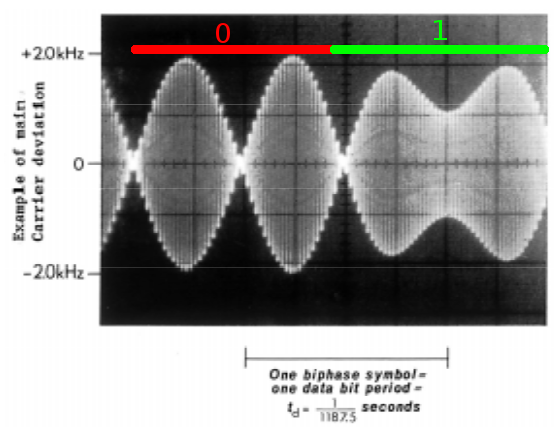
\includegraphics[width=1\linewidth]{gfx/rds/rds_waveform.png}
	\caption{RDS envelope waveform after Frequency demodulation. \cite{1999:iec62106}}
	\label{fig:rds_envelope}
\end{figure}



\subsection{RDS coding scheme}

RDS frames are called groups and each group consists of 4 blocks called
A, B, C and D. One block has a length of 16 bit plus a 10 bit checkword.
Block A always contains the \ac{PI} which identifies the radio station.
The content of the other blocks depends on the group type which is located
in block B (see \autoref{fig:rds_group0A}).

\begin{figure}
	\centering
	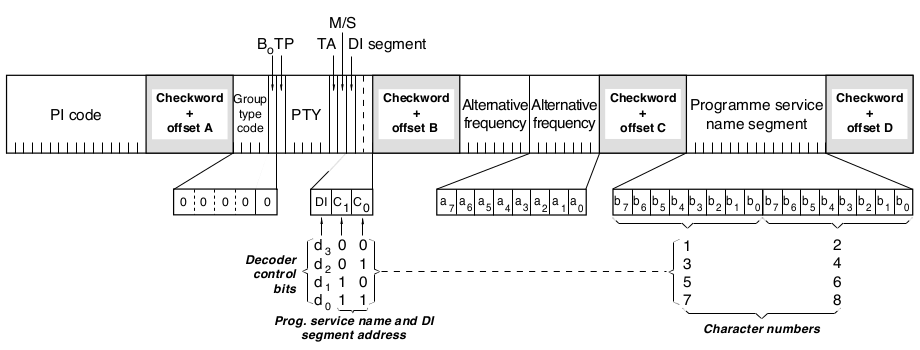
\includegraphics[width=1\linewidth]{gfx/rds/group0A.png}
	\caption{Coding scheme of RDS: group 0A. \cite{1999:iec62106}}
	\label{fig:rds_group0A}
\end{figure}

\begin{table}
	\begin{center}
		\begin{tabular}{ c c l }
		 Group Type & Group Version & Description \\\hline
		 0 & A & Basic tuning and switching information only \\
		 0 & B & Basic tuning and switching information only \\
		 1 & A & Programme Item Number and slow labelling codes\\
		 1 & B & Programme Item Number \\
		 2 & A & RadioText only \\
		 2 & B & RadioText only \\
		 3 & A & Applications Identification for ODA only \\
		 3 & B & Open Data Applications\\
		 4 & A & Clock-time and date only \\
		 4 & B & Open Data Applications\\
		 5 & A & Transparent Data Channels \\
		 5 & B & Transparent Data Channels \\
		 6 & A & In House applications or ODA \\
		 6 & B & In House applications or ODA \\
		 7 & A & Radio Paging or ODA \\
		 7 & B & Open Data Applications\\
		 8 & A & Traffic Message Channel or ODA \\
		 8 & B & Open Data Applications\\
		 9 & A & Emergency Warning System or ODA \\
		 9 & B & Open Data Applications\\
		10 & A & Programme Type Name\\
		10 & B & Open Data Applications\\
		11 & A & Open Data Applications\\
		11 & B & Open Data Applications\\
		12 & A & Open Data Applications\\
		12 & B & Open Data Applications\\
		13 & A & Enhanced Radio Paging or ODA\\
		13 & B & Open Data Applications\\
		14 & A & Enhanced Other Networks information only \\
		14 & B & Enhanced Other Networks information only \\
		15 & A & Defined in RBDS [15] only\\
		15 & B & Fast switching information only \\\hline
		\end{tabular}
		\caption{RDS Group Types}
		\label{tab:rds_groups}
	\end{center}
\end{table}

\autoref{tab:rds_groups} lists all group types and their descriptions.
The \ac{RDS} demodulation in AnSiAn only decodes types 0 and 2 because they contain
the basic information which is also often displayed on the radio
receiver.


\subsection{Evaluation in Octave}

Developing a signal processing application on Android has many drawbacks. One
issue is that it is very hard to debug the actuall signal processing components
because of the lack of proper tools to visualize and analyze the data that is
being processed. It is also not possible to do rapid prototyping without
sufficient signal processing libaries available. Therefore the \ac{RDS}
demodulator was first developed in Octave and afterwards ported to Android.

For development and testing it is better to work on recorded samples instead
of live captures. This makes tests reproducable and simplify the development
environment. The file was recorded using the record feature of RF Analyzer. It
can be imported to Octave by using the \emph{read\_cuchar\_binary()} script
provided by the GNU Radio project. After each step the produced output data
can be written back to an \emph{IQ} in order to use it in the Android application.
This way it is possible to develop each component of the demodulation process
separately and the output can be visualized on the developing machine.

The demodulation is done in the following steps:
\begin{enumerate}
	\item Downmixing the radio signal to baseband and filter it (see 
		\autoref{fig:rds_downmixing}).
	\item \ac{FM} demodulation (see \autoref{fig:quad_demod_spectrum}).
	\item Downmixing the \ac{RDS} signal to baseband and filter it
		(see \autoref{fig:rds_extraction} b and c).
	\item Take the absolute value of the signal to get the envelope
		that was shown above (see \autoref{fig:rds_waveform}).
	\item Find the beginning of a symbol by searching for a minimum in
		the waveform. From there find the end of the symbol with the
		same strategy. Now determine whether the symbol is a one or a
		zero according to the value of the minimum found in the middle
		of the sample compared to its peaks.
\end{enumerate}

\begin{figure}
\subfloat[Spectrum of the captured signal]{%
  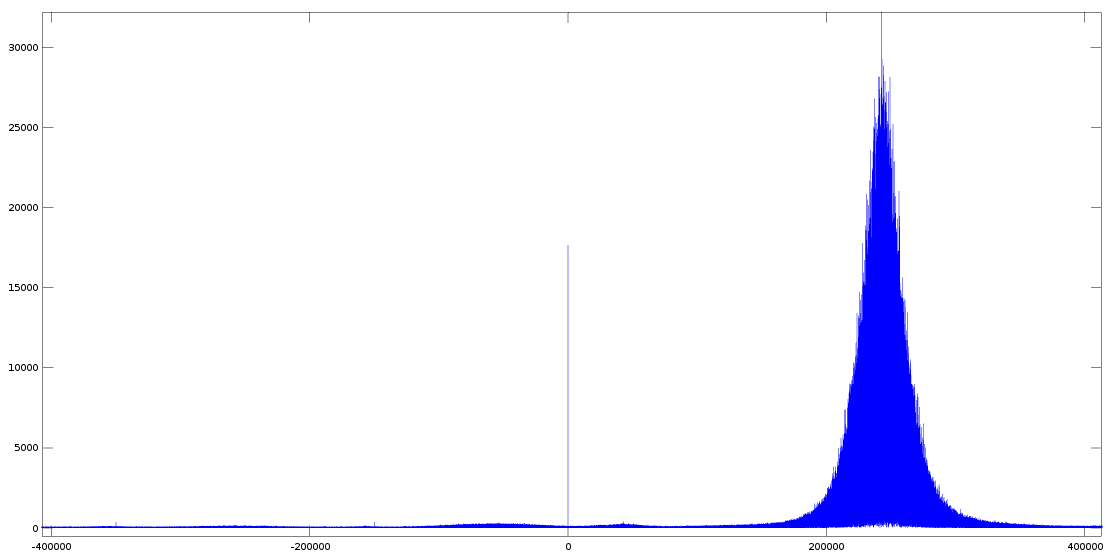
\includegraphics[clip,width=1\linewidth]{gfx/rds/raw_signal_spectrum.png}%
}

\subfloat[Spectrum after downmixing and filtering]{%
  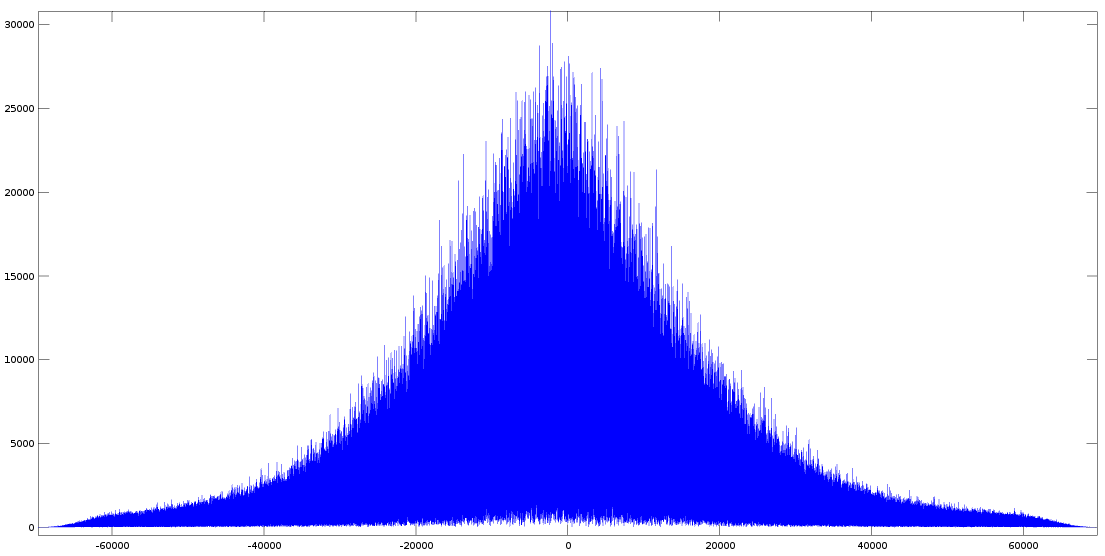
\includegraphics[clip,width=1\linewidth]{gfx/rds/fm_baseband_filtered_spectrum.png}%
}
\caption{FM Modulated Signal}
\label{fig:rds_downmixing}
\end{figure}


\begin{figure}
\subfloat[Signal spectrum after FM demodulation]{%
  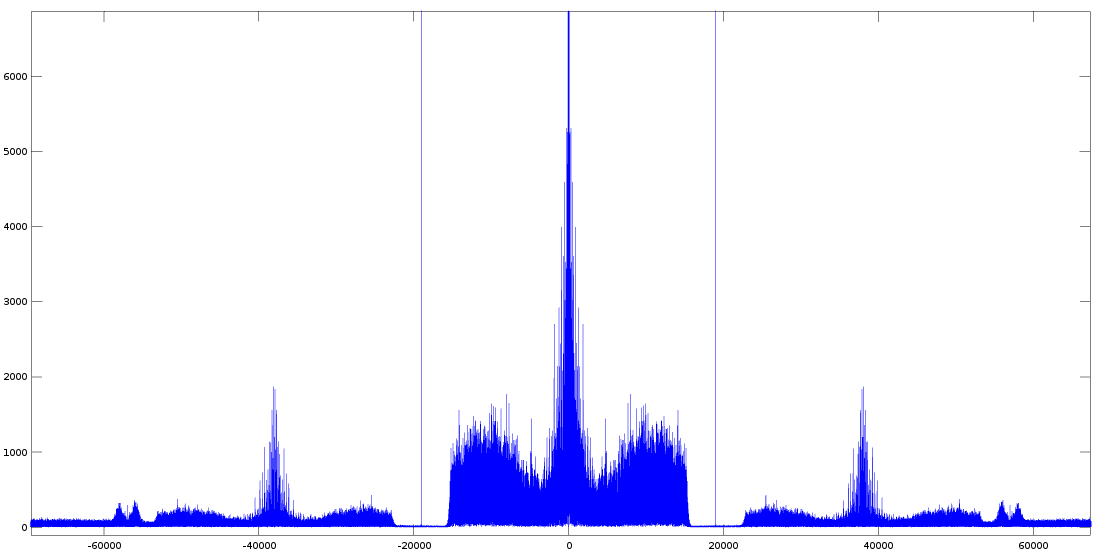
\includegraphics[clip,width=1\linewidth]{gfx/rds/quad_demod_spectrum.png}%
  \label{fig:quad_demod_spectrum}
}

\subfloat[RDS baseband spectrum after downmixing]{%
  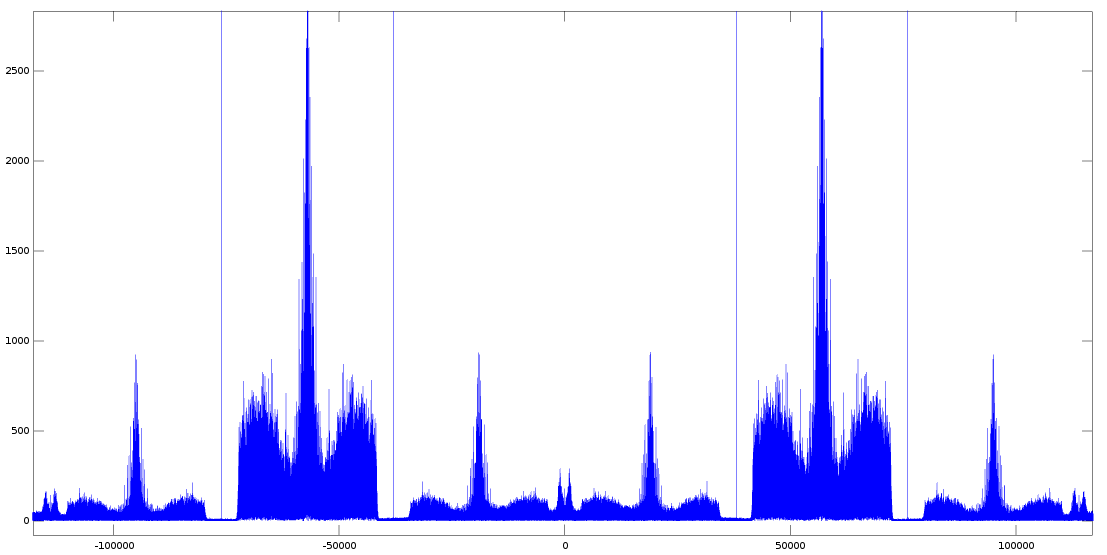
\includegraphics[clip,width=1\linewidth]{gfx/rds/rds_baseband_unfiltered_spectrum.png}%
}

\subfloat[RDS baseband spectrum after filtering]{%
  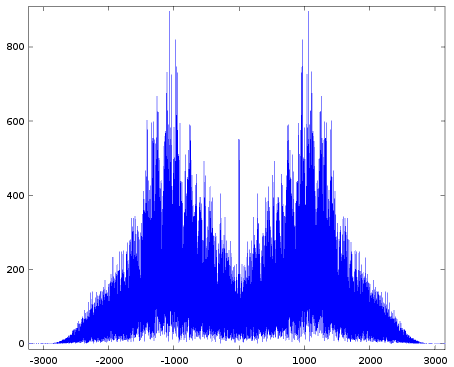
\includegraphics[clip,width=1\linewidth]{gfx/rds/rds_baseband_spectrum.png}%
}
\caption{Extracting the RDS signal from the FM signal}
\label{fig:rds_extraction}
\end{figure}

\begin{figure}
	\centering
	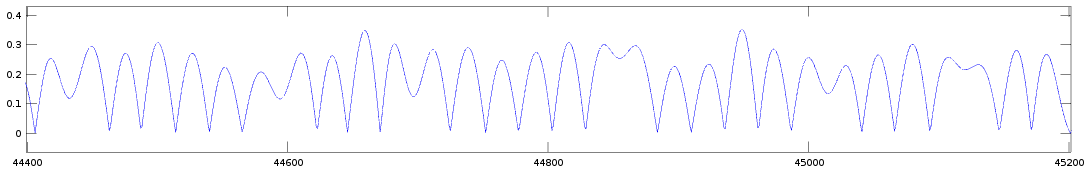
\includegraphics[width=1\linewidth]{gfx/rds/rds_magnitude_waveform.png}
	\caption{RDS waveform after take the absolute values}
	\label{fig:rds_waveform}
\end{figure}

The octave code used to execute the steps mentioned above is shown in the
listing below:

\begin{lstlisting}[label=lst:octave_rds, caption=Octave implementation of the RDS demodulator, language=none]
signal = read_cuchar_binary ("~/Downloads/2016-06-01-20-17-18_rtlsdr_100550000Hz_1000000Sps.iq" );
t = linspace(0, length(signal)/1000000, length(signal))';
carrier = e.^(2*pi*-245000*t*i);
down = carrier .* signal;
fl = fir1(300, 100000/1000000*2);
filtered = filter(fl, 1, down);
demod = quad_demod(filtered, 1);
t2 = linspace(0, length(demod)/1000000, length(demod));
rdscarrier = cos(2*pi*-57000*t2)';
rdsbase = demod(1:length(rdscarrier)) .* rdscarrier ;
frds = fir1(300, 2400/1000000*2);
rdsbase_filtered = filter(frds,1,rdsbase);
downsampled = decimate(rdsbase_filtered, 16).*80;
write_cuchar_binary (downsampled, "~/Downloads/rds_baseband_62500sps.iq");
bits = rds_bpsk_demodulate(downsampled, 62500);
rds_decode(bits)
\end{lstlisting}

The \emph{quad\_demod()} function does the quadrature demodulation
(FM demodulation). The \emph{rds\_bpsk\_demodulate()} function is shown
in the following listing:

\begin{lstlisting}[label=lst:octave_rds_bpsk, caption=Octave implementation of the BPSK demodulation, language=none]
function demod = rds_bpsk_demodulate(signal, fs)
  samples_per_symbol = fs/1187.5
  samples_per_symbol = ceil(samples_per_symbol)
  envelope = abs(signal);
  
  % Find the first minimum
  [minimum, idx1] = min(envelope(1:samples_per_symbol))
  
  bits = [];
  while (idx1 + samples_per_symbol*2 < length(envelope))
    % find end of symbol idx2 (minimum near idx1 + samples_per_symbol)
    from = round(idx1+samples_per_symbol*0.75);
    to   = round(idx1+samples_per_symbol*1.25);
    [minimum, idx2] = min(envelope(from:to));
    idx2 = idx2 + from;
    
    % calc mean of all samples between idx1 and idx2 and calc threshold = mean/2
    m = mean(envelope(idx1:idx2));
    threshold = m/2;
    
    % get minimum sample in the middle between idx1 and idx2 ...
    span = idx2 - idx1;
    from = round((idx1+idx2)*0.5 - 0.25*span);
    to   = round((idx1+idx2)*0.5 + 0.25*span);
    [minimum, idxmiddle] = min(envelope(from:to));
    idxmiddle = idxmiddle + from;
    
    % Check whether we have the correct timing. It might be, that idx2 is
    % actually in the middle of a symbol than at its end.
    if (envelope(idx2) > threshold)
      % In this case we find the minimum between idx1 and idx2 and set it
      % as idx1 for the next round:
      %printf("WARNING: Wrong timing. thres=%f < envelope(idx2=%d)=%f\n",threshold,idx2,envelope(idx2));
      idx1 = idxmiddle;
      continue;
    endif
    
    % ... and check it against the threshold
    s = envelope(idxmiddle);
    if (s > threshold)
      bits = [bits 1];
    else
      bits = [bits 0];
    endif
    
    % idx1 = idx2 and continue with the next symbol..
    idx1 = idx2;
    
  endwhile
  demod = bits;
\end{lstlisting}


\subsection{Android Implementation}

For the Android implementation two classes are added to the AnSiAn codebase:
\begin{itemize}
	\item BPSK: This class handles the \ac{BPSK} demodulation and can be
		reused by other demodulators using the \ac{BPSK} modulation scheme
		(e.g. PSK31).
	\item RDS: This class integrates in the existing FM class for frequency
		demodulation. It handles the decoding and processing of \ac{RDS}
		groups. 
\end{itemize}

A screenshot of the application demodulating the \ac{RDS} signal of the
\emph{Antenne Frankfurt} station is shown in \autoref{fig:rds_android_screenshot}.

\begin{figure}
	\centering
	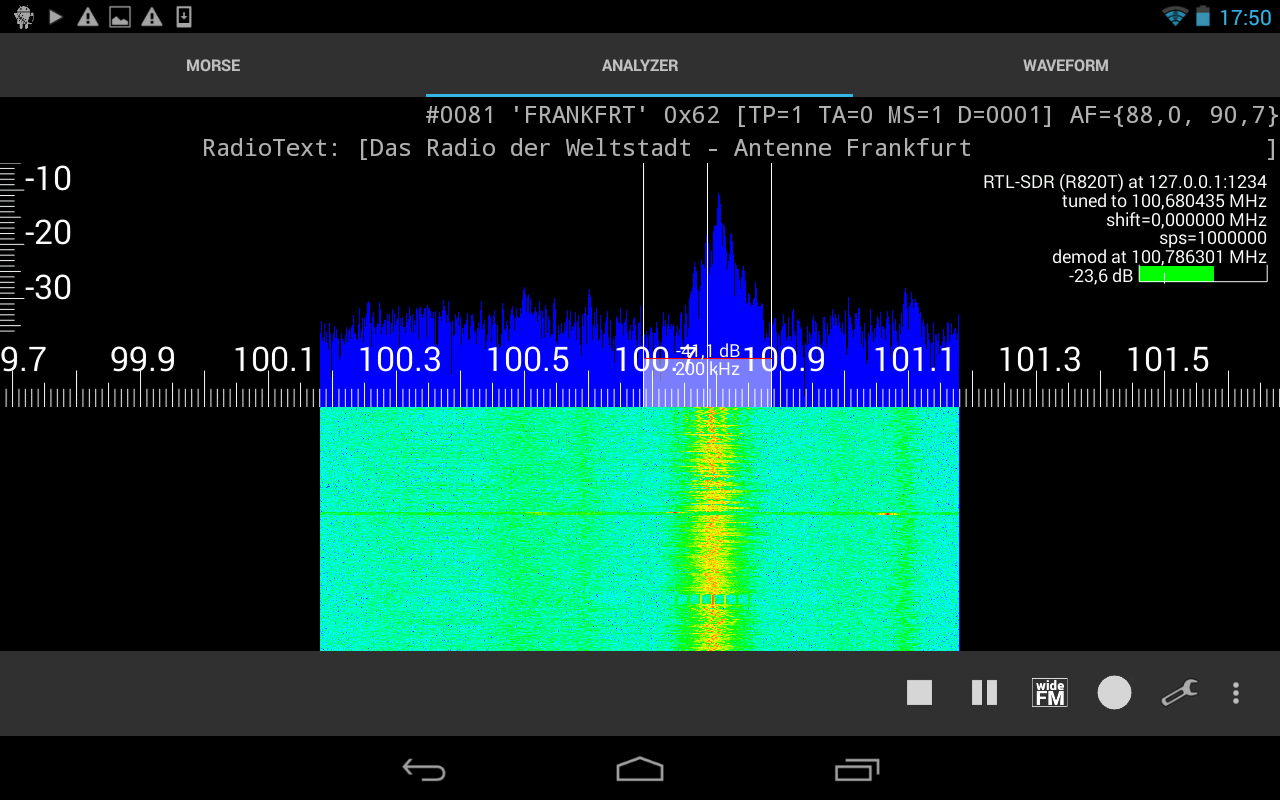
\includegraphics[width=1\linewidth]{gfx/rds/android_screenshot.png}
	\caption{Screenshot of the RDS demodulator on a Nexus 7}
	\label{fig:rds_android_screenshot}
\end{figure}


%************************************************
%\chapter{Evaluation}\label{ch:evaluation} % $\mathbb{ZNR}$
%************************************************
%\glsresetall % Resets all acronyms to not used

